\documentclass[sigconf]{acmart}
\usepackage{amssymb}
\usepackage{setspace}
\usepackage{tikz}
\usetikzlibrary{arrows.meta}

\copyrightyear{2019}
\acmYear{2019}
\setcopyright{rightsretained}
\acmConference[]{---}{---}{---}
%\acmBooktitle{}
%\acmPrice{15.00}
%\acmDOI{}
%\acmISBN{}

\begin{document}
\title{Interleaving Anomalies in Collaborative Text Editors}

\author{Martin Kleppmann}
\email{mk428@cl.cam.ac.uk}
\orcid{0000-0001-7252-6958}
\affiliation{%
  \institution{University of Cambridge}
  \streetaddress{William Gates Building, 15 JJ Thomson Avenue}
  \city{Cambridge}
  \state{}
  \postcode{CB3 0FD}
  \country{UK}
}

\author{Victor B.\ F.\ Gomes}
\email{vb358@cl.cam.ac.uk}
\orcid{0000-0002-2954-4648}
\affiliation{%
  \institution{University of Cambridge}
  \streetaddress{William Gates Building, 15 JJ Thomson Avenue}
  \city{Cambridge}
  \state{}
  \postcode{CB3 0FD}
  \country{UK}
}

\author{Dominic P.\ Mulligan}
\email{Dominic.Mulligan@arm.com}
\orcid{0000-0003-4643-3541}
\affiliation{%
  \institution{Arm Research}
  \city{Cambridge}
  \country{UK}
}

\author{Alastair R.\ Beresford}
\email{arb33@cl.cam.ac.uk}
\orcid{0000-0003-0818-6535}
\affiliation{%
  \institution{University of Cambridge}
  \streetaddress{William Gates Building, 15 JJ Thomson Avenue}
  \city{Cambridge}
  \state{}
  \postcode{CB3 0FD}
  \country{UK}
}

\begin{abstract}
TODO
\end{abstract}

%
% The code below is generated by the tool at http://dl.acm.org/ccs.cfm.
% Please copy and paste the code instead of the example below.
%
\begin{CCSXML}
\end{CCSXML}

\keywords{TODO}
\maketitle

\section{Introduction}

In collaborative software, several users may contribute to a project by creating and editing shared documents, such as text documents, spreadsheets, graphics files, or presentations.
When a user wishes to view a document, a copy of that document is loaded on the user's computer (e.g.\ in a tab of their web browser, or in a native app on their device).
When a user wishes to modify a document, their changes are immediately applied to the copy of the document on the user's computer, and then asynchronously sent to any other users who have a copy of the document (possibly via a server, which may also store a copy).
This collaboration scenario is very similar to the problem of replication in distributed databases: in this context, the shared data is a database rather than a document, and each node that has a copy of the data is called a \emph{replica}.

At a high level, there are two possible ways of managing modifications to documents: either the system enforces that only one user at a time may edit a particular document (for example by obtaining a lock on the file before allowing any modifications), or the system allows multiple users to edit a document concurrently.
The latter case is known as \emph{optimistic replication}.
In an optimistic replication setting, it can happen that several users make changes at the same time, leading the state of these users' documents to diverge.
This is illustrated in Figure~\ref{fig:hello-world}, where one user changes the document \texttt{`Hello!'} to \texttt{`Hello World!'}, while another user concurrently changes it to \texttt{`Hello! :)'}.
In order to ensure that no user input is lost, these concurrent changes must be merged into a consistent document~-- in this example, \texttt{`Hello World! :)'}.

\begin{figure*}
  \centering
  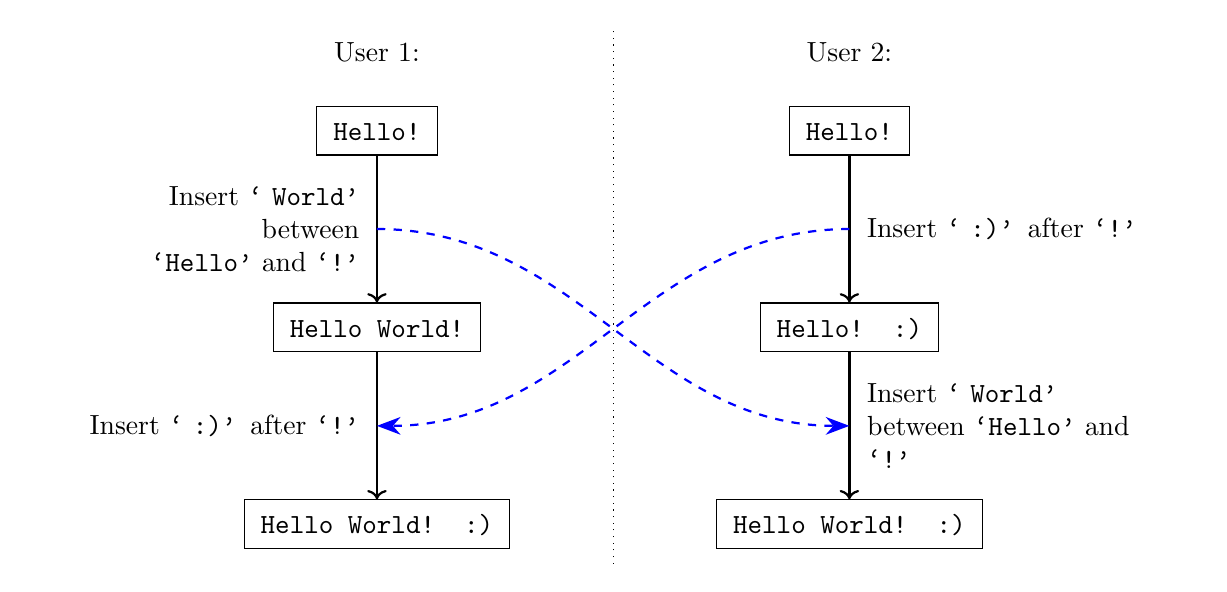
\begin{tikzpicture}[auto,scale=1.0]
    \tikzstyle{box}=[rectangle,draw,inner xsep=6pt,text height=9pt,text depth=2pt]
	\tikzstyle{leftevent}=[left,inner xsep=6pt,text width=4cm,text ragged left,midway]
	\tikzstyle{rightevent}=[right,inner xsep=6pt,text width=4cm,text ragged,midway]
	\tikzstyle{time}=[thick,->]
	\tikzstyle{network}=[thick,dashed,blue,-{Stealth[length=3mm]}]
	\node (left0)  at (0,6.0) {User 1:};
	\node (left1)  at (0,5.0) [box] {\texttt{Hello!}};
	\node (left2)  at (0,2.5) [box] {\texttt{Hello World!}};
	\node (left3)  at (0,0.0) [box] {\texttt{Hello World! :)}};
	\node (right0) at (6,6.0) {User 2:};
	\node (right1) at (6,5.0) [box] {\texttt{Hello!}};
	\node (right2) at (6,2.5) [box] {\texttt{Hello! :)}};
	\node (right3) at (6,0.0) [box] {\texttt{Hello World! :)}};
	\draw [time] (left1)  -- (left2)  node (send1) [leftevent]  {Insert \texttt{`~World'}\\between \texttt{`Hello'} and \texttt{`!'}};
	\draw [time] (right1) -- (right2) node (send2) [rightevent] {Insert \texttt{` :)'} after \texttt{`!'}};
    \draw [time] (left2)  -- (left3)  node (recv2) [leftevent]  {Insert \texttt{` :)'} after \texttt{`!'}};
    \draw [time] (right2) -- (right3) node (recv1) [rightevent] {Insert \texttt{`~World'}\\between \texttt{`Hello'} and \texttt{`!'}};
    \draw [network] (send1.east) to [out=0,in=180] (recv1.west);
    \draw [network] (send2.west) to [out=180,in=0] (recv2.east);
	\path [draw,dotted] (3,-0.5) -- (3,6.3);
  \end{tikzpicture}
  \caption{Simple example of concurrent text editing. Solid black lines indicate state changes over time, while dashed blue arrows indicate network communication.}
  \label{fig:hello-world}
\end{figure*}

This kind of merge can either be performed manually (the approach employed by most version control systems, such as git), or it can be automated.
Conflict-free Replicated Data Types, or CRDTs~\cite{Shapiro:2011wy,Shapiro:2011un}, have been developed to automate such merges.
A CRDT is an abstract datatype whose state can be modified by performing certain operations (for example, a datatype for text editing may allow characters to be inserted or deleted anywhere in the document).
It allows arbitrary operations to be performed on different replicas; either the updated state or the operations or the operations are then sent over the network and applied or merged into copies of the document on other replicas.

\subsection{Consistency for Optimistic Replication}

CRDTs provide a consistency model called \emph{strong eventual consistency}~\cite{Shapiro:2011un,Gomes:2017gy}, which is defined by the following properties:
\begin{description}
\item[Eventual delivery]: An update applied on one correct replica is eventually applied on all correct replicas.
\item[Convergence]: If the same set of updates have been applied on two replicas, those replicas have equivalent state.
\item[Termination]: All method executions terminate.
\end{description}
In operation-based CRDTs the convergence property is implemented by ensuring that concurrent operations commute.
For example, in Figure~\ref{fig:hello-world}, User 1 first applies the insertion of \texttt{` World'} and then the insertion of \texttt{` :)'}, while User 2 applies the insertions in the opposite order.
Commutativity of the insertion ensures that the outcome is the same in both cases.

When replicas mutually merge each others' changes, the convergence property ensures that those replicas end up in the same state.
However, nothing so far has specified what that state should be.
This means that, although strong eventual consistency is necessary, it is not sufficient, as it does not capture all of the consistency properties that we require in a collaborative application.

In this paper we examine a particular consistency property for collaborative text editors that has so far been overlooked in the literature.
A failure to satisfy this property may result in arbitrary text interleaving, potentially resulting in an undesirable document state.
We highlight existing CRDT algorithms and a specification that exhibit this anomaly, and compare them to other approaches that do not suffer from this anomaly, or only a lesser variant.


\section{The Interleaving Anomaly}


\begin{figure*}
  \centering
  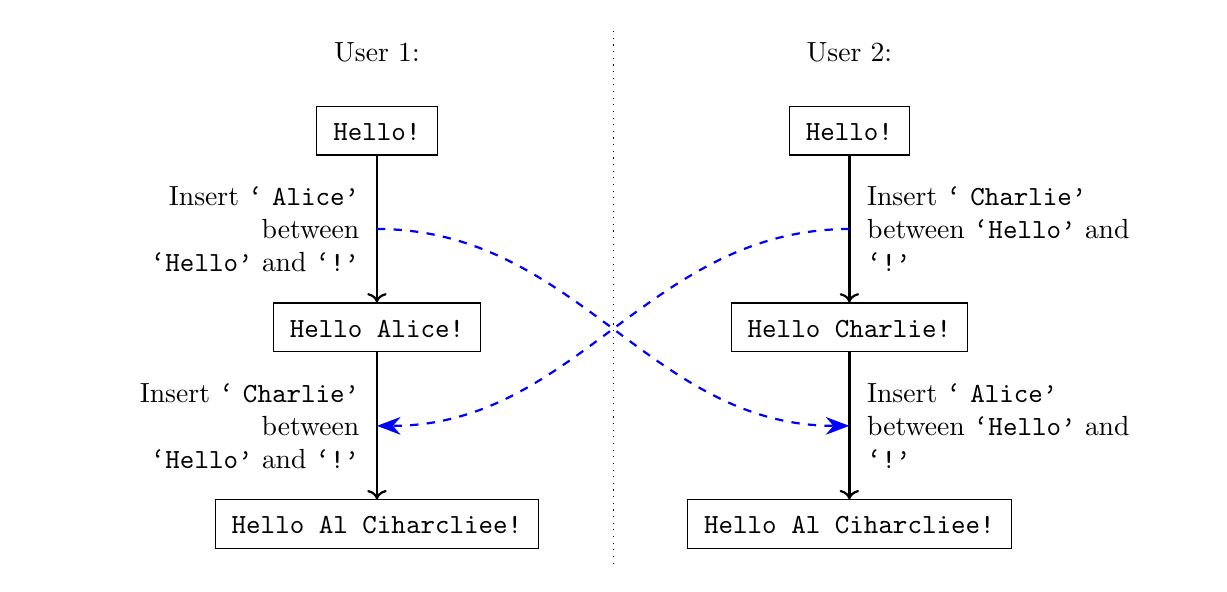
\begin{tikzpicture}[auto,scale=1.0]
    \tikzstyle{box}=[rectangle,draw,inner xsep=6pt,text height=9pt,text depth=2pt]
	\tikzstyle{leftevent}=[left,inner xsep=6pt,text width=4cm,text ragged left,midway]
	\tikzstyle{rightevent}=[right,inner xsep=6pt,text width=4cm,text ragged,midway]
	\tikzstyle{time}=[thick,->]
	\tikzstyle{network}=[thick,dashed,blue,-{Stealth[length=3mm]}]
	\node (left0)  at (0,6.0) {User 1:};
	\node (left1)  at (0,5.0) [box] {\texttt{Hello!}};
	\node (left2)  at (0,2.5) [box] {\texttt{Hello Alice!}};
	\node (left3)  at (0,0.0) [box] {\texttt{Hello Al Ciharcliee!}};
	\node (right0) at (6,6.0) {User 2:};
	\node (right1) at (6,5.0) [box] {\texttt{Hello!}};
	\node (right2) at (6,2.5) [box] {\texttt{Hello Charlie!}};
	\node (right3) at (6,0.0) [box] {\texttt{Hello Al Ciharcliee!}};
	\draw [time] (left1)  -- (left2)  node (send1) [leftevent]  {Insert \texttt{`~Alice'}\\between \texttt{`Hello'} and \texttt{`!'}};
	\draw [time] (right1) -- (right2) node (send2) [rightevent] {Insert \texttt{`~Charlie'}\\between \texttt{`Hello'} and \texttt{`!'}};
    \draw [time] (left2)  -- (left3)  node (recv2) [leftevent]  {Insert \texttt{`~Charlie'}\\between \texttt{`Hello'} and \texttt{`!'}};
    \draw [time] (right2) -- (right3) node (recv1) [rightevent] {Insert \texttt{`~Alice'}\\between \texttt{`Hello'} and \texttt{`!'}};
    \draw [network] (send1.east) to [out=0,in=180] (recv1.west);
    \draw [network] (send2.west) to [out=180,in=0] (recv2.east);
	\path [draw,dotted] (3,-0.5) -- (3,6.3);
  \end{tikzpicture}
  \caption{Two concurrent insertions at the same position are interleaved.}
  \label{fig:bad-merge}
\end{figure*}

\begin{figure*}
  \centering
  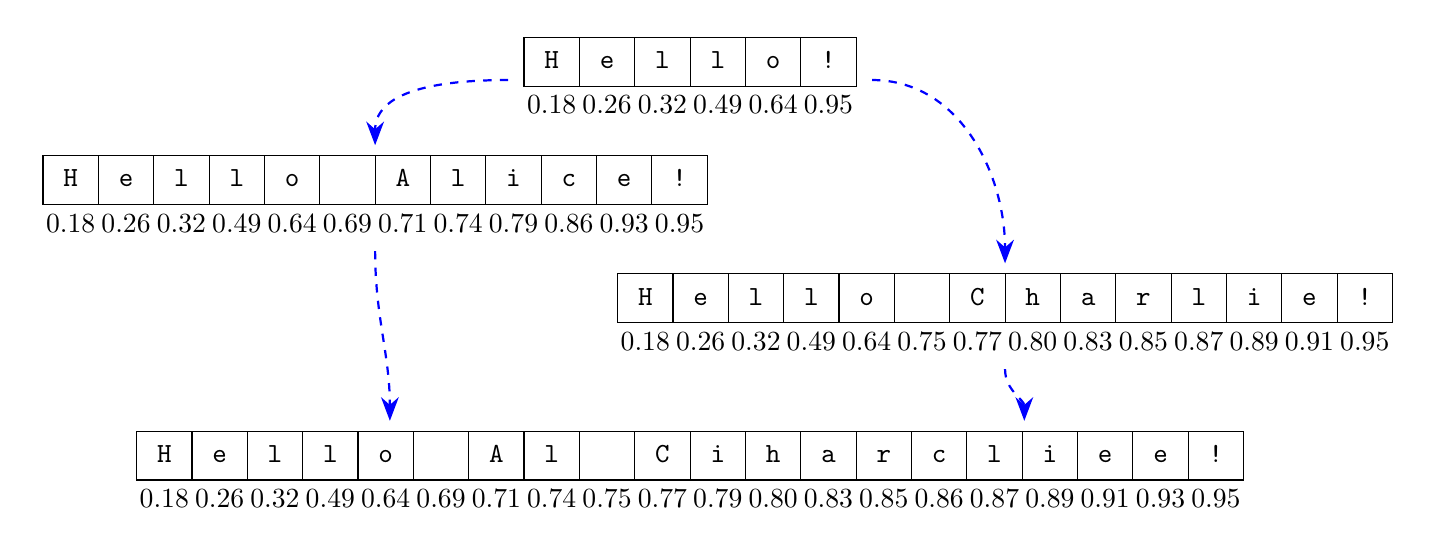
\begin{tikzpicture}[auto,scale=1.0]
    \tikzstyle{box}=[rectangle,draw,inner xsep=6pt,text height=9pt,text depth=2pt]
	\tikzstyle{state}=[matrix,column sep={20pt,between origins}]
	\tikzstyle{val}=[draw,anchor=base,minimum width=20pt,text height=8pt,text depth=3pt]
	\tikzstyle{oid}=[anchor=base]
	\tikzstyle{leftevent}=[left,inner xsep=6pt,text width=4cm,text ragged left,midway]
	\tikzstyle{rightevent}=[right,inner xsep=6pt,text width=4cm,text ragged,midway]
	\tikzstyle{time}=[thick,->]
	\tikzstyle{network}=[thick,dashed,blue,-{Stealth[length=3mm]}]
	\node (hello) at (4,5) [state] {
		\node [val] {\texttt{H}}; &
		\node [val] {\texttt{e}}; &
		\node [val] {\texttt{l}}; &
		\node [val] {\texttt{l}}; &
		\node [val] {\texttt{o}}; &
		\node [val] {\texttt{!}}; \\
		\node [oid] {0.18}; & % H
		\node [oid] {0.26}; & % e
		\node [oid] {0.32}; & % l
		\node [oid] {0.49}; & % l
		\node [oid] {0.64}; & % o
		\node [oid] {0.95}; \\ % !
	};
	\node (alice) at (0,3.5) [state] {
		\node [val] {\texttt{H}}; &
		\node [val] {\texttt{e}}; &
		\node [val] {\texttt{l}}; &
		\node [val] {\texttt{l}}; &
		\node [val] {\texttt{o}}; &
		\node [val] {\texttt{ }}; &
		\node [val] {\texttt{A}}; &
		\node [val] {\texttt{l}}; &
		\node [val] {\texttt{i}}; &
		\node [val] {\texttt{c}}; &
		\node [val] {\texttt{e}}; &
		\node [val] {\texttt{!}}; \\
		\node [oid] {0.18}; & % H
		\node [oid] {0.26}; & % e
		\node [oid] {0.32}; & % l
		\node [oid] {0.49}; & % l
		\node [oid] {0.64}; & % o
		\node [oid] {0.69}; & %
		\node [oid] {0.71}; & % A
		\node [oid] {0.74}; & % l
		\node [oid] {0.79}; & % i
		\node [oid] {0.86}; & % c
		\node [oid] {0.93}; & % e
		\node [oid] {0.95}; \\ % !
	};
	\node (charlie) at (8,2) [state] {
		\node [val] {\texttt{H}}; &
		\node [val] {\texttt{e}}; &
		\node [val] {\texttt{l}}; &
		\node [val] {\texttt{l}}; &
		\node [val] {\texttt{o}}; &
		\node [val] {\texttt{ }}; &
		\node [val] {\texttt{C}}; &
		\node [val] {\texttt{h}}; &
		\node [val] {\texttt{a}}; &
		\node [val] {\texttt{r}}; &
		\node [val] {\texttt{l}}; &
		\node [val] {\texttt{i}}; &
		\node [val] {\texttt{e}}; &
		\node [val] {\texttt{!}}; \\
		\node [oid] {0.18}; & % H
		\node [oid] {0.26}; & % e
		\node [oid] {0.32}; & % l
		\node [oid] {0.49}; & % l
		\node [oid] {0.64}; & % o
		\node [oid] {0.75}; & %
		\node [oid] {0.77}; & % C
		\node [oid] {0.80}; & % h
		\node [oid] {0.83}; & % a
		\node [oid] {0.85}; & % r
		\node [oid] {0.87}; & % l
		\node [oid] {0.89}; & % i
		\node [oid] {0.91}; & % e
		\node [oid] {0.95}; \\ % !
	};
	\node (interleaved) at (4,0) [state] {
		\node [val] {\texttt{H}}; &
		\node [val] {\texttt{e}}; &
		\node [val] {\texttt{l}}; &
		\node [val] {\texttt{l}}; &
		\node [val] {\texttt{o}}; &
		\node [val] {\texttt{ }}; &
		\node [val] {\texttt{A}}; &
		\node [val] {\texttt{l}}; &
		\node [val] {\texttt{ }}; &
		\node [val] {\texttt{C}}; &
		\node [val] {\texttt{i}}; &
		\node [val] {\texttt{h}}; &
		\node [val] {\texttt{a}}; &
		\node [val] {\texttt{r}}; &
		\node [val] {\texttt{c}}; &
		\node [val] {\texttt{l}}; &
		\node [val] {\texttt{i}}; &
		\node [val] {\texttt{e}}; &
		\node [val] {\texttt{e}}; &
		\node [val] {\texttt{!}}; \\
		\node [oid] {0.18}; & % H
		\node [oid] {0.26}; & % e
		\node [oid] {0.32}; & % l
		\node [oid] {0.49}; & % l
		\node [oid] {0.64}; & % o
		\node [oid] {0.69}; & %
		\node [oid] {0.71}; & % A
		\node [oid] {0.74}; & % l
		\node [oid] {0.75}; & %
		\node [oid] {0.77}; & % C
		\node [oid] {0.79}; & % i
		\node [oid] {0.80}; & % h
		\node [oid] {0.83}; & % a
		\node [oid] {0.85}; & % r
		\node [oid] {0.86}; & % c
		\node [oid] {0.87}; & % l
		\node [oid] {0.89}; & % i
		\node [oid] {0.91}; & % e
		\node [oid] {0.93}; & % e
		\node [oid] {0.95}; \\ % !
	};
	\draw [network] (hello.west)    to [out=180,in=90] (alice.north);
	\draw [network] (hello.east)    to [out=0,in=90]   (charlie.north);
	\draw [network] (alice.south)   to [out=270,in=90] (interleaved.170);
	\draw [network] (charlie.south) to [out=270,in=90] (interleaved.9);
  \end{tikzpicture}
  \caption{Interleaving occurs because characters are assigned positions in a dense identifier space, e.g.\ the real numbers $\mathbb{R}$.}
  \label{fig:real-numbers}
\end{figure*}

\begin{figure*}
  \centering
  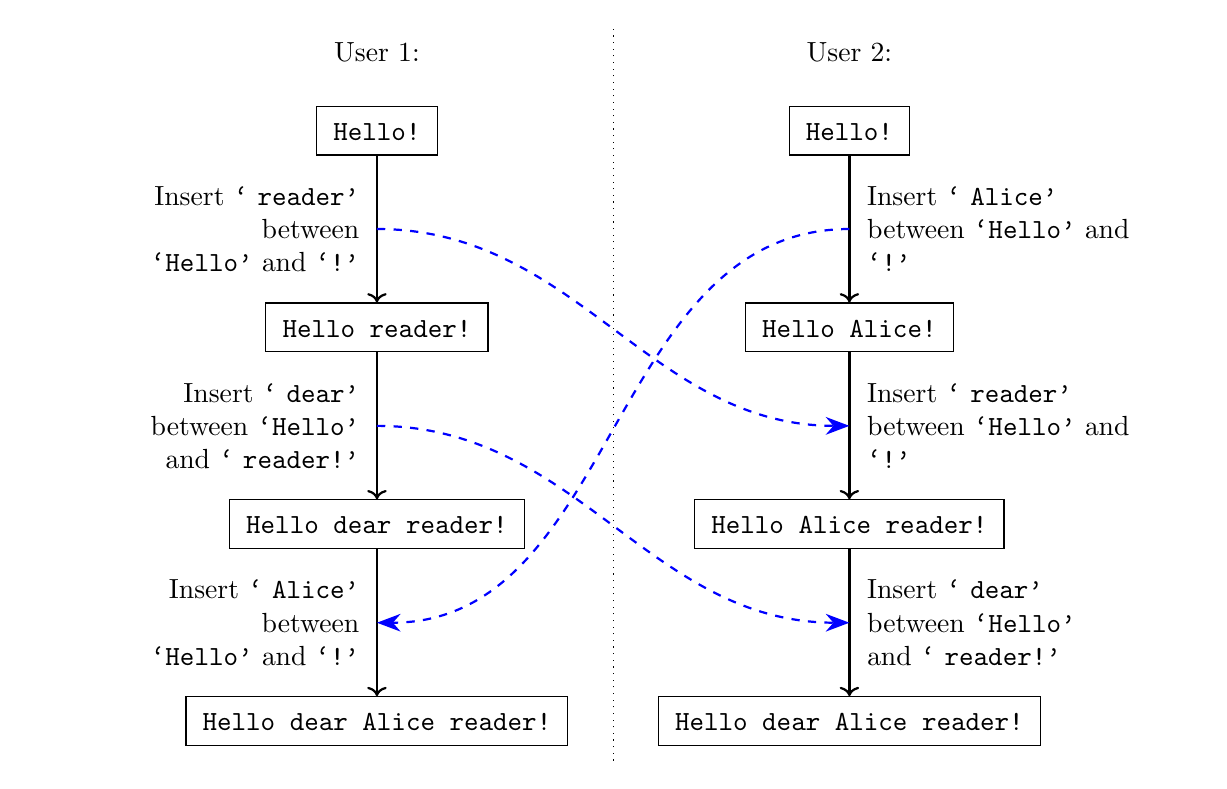
\begin{tikzpicture}[auto,scale=1.0]
    \tikzstyle{box}=[rectangle,draw,inner xsep=6pt,text height=9pt,text depth=2pt]
	\tikzstyle{leftevent}=[left,inner xsep=6pt,text width=4cm,text ragged left,midway]
	\tikzstyle{rightevent}=[right,inner xsep=6pt,text width=4cm,text ragged,midway]
	\tikzstyle{time}=[thick,->]
	\tikzstyle{network}=[thick,dashed,blue,-{Stealth[length=3mm]}]
	\node (left0)  at (0,8.5) {User 1:};
	\node (left1)  at (0,7.5) [box] {\texttt{Hello!}};
	\node (left2)  at (0,5.0) [box] {\texttt{Hello reader!}};
	\node (left3)  at (0,2.5) [box] {\texttt{Hello dear reader!}};
	\node (left4)  at (0,0.0) [box] {\texttt{Hello dear Alice reader!}};
	\node (right0) at (6,8.5) {User 2:};
	\node (right1) at (6,7.5) [box] {\texttt{Hello!}};
	\node (right2) at (6,5.0) [box] {\texttt{Hello Alice!}};
	\node (right3) at (6,2.5) [box] {\texttt{Hello Alice reader!}};
	\node (right4) at (6,0.0) [box] {\texttt{Hello dear Alice reader!}};
	\draw [time] (left1)  -- (left2)  node (send1) [leftevent]  {Insert \texttt{`~reader'}\\between \texttt{`Hello'} and \texttt{`!'}};
    \draw [time] (left2)  -- (left3)  node (send2) [leftevent]  {Insert \texttt{`~dear'}\\between \texttt{`Hello'}\\and \texttt{` reader!'}};
    \draw [time] (left3)  -- (left4)  node (recv3) [leftevent]  {Insert \texttt{`~Alice'}\\between \texttt{`Hello'} and \texttt{`!'}};
	\draw [time] (right1) -- (right2) node (send3) [rightevent] {Insert \texttt{`~Alice'}\\between \texttt{`Hello'} and \texttt{`!'}};
    \draw [time] (right2) -- (right3) node (recv1) [rightevent] {Insert \texttt{`~reader'}\\between \texttt{`Hello'} and \texttt{`!'}};
    \draw [time] (right3) -- (right4) node (recv2) [rightevent] {Insert \texttt{`~dear'}\\between \texttt{`Hello'}\\and \texttt{` reader!'}};
    \draw [network] (send1.east) to [out=0,in=180] (recv1.west);
    \draw [network] (send2.east) to [out=0,in=180] (recv2.west);
    \draw [network] (send3.west) to [out=180,in=0] (recv3.east);
	\path [draw,dotted] (3,-0.5) -- (3,8.8);
  \end{tikzpicture}
  \caption{The lesser interleaving anomaly that can occur with RGA.}
  \label{fig:rga-interleaving}
\end{figure*}



\begin{acks}
This work was supported by The Boeing Company and the EPSRC ``REMS: Rigorous Engineering for Mainstream Systems'' programme grant (EP/K008528).
\end{acks}

\bibliographystyle{ACM-Reference-Format}
\bibliography{references}
\end{document}
